\section{Internet Protocol}
IP(Internet Protocol)はTCP/IPモデルにおいてデータの送受信を担うプロトコルである.OSI参照モデルにおけるレイヤ3(ネットワーク層)に相当する役割を持ち,IPアドレスと呼ばれるIP独自の論理アドレスに基づいてデータをやり取りすることを特徴としている.IPは異なるネットワークに属する通信相手までデータを届ける機能を持ち,物理的に遠く離れた相手との通信経路を確立する.TCP/IPモデルの中核となる重要なプロトコルである.

\subsection{IPアドレスとは}
IPアドレスはIPでの通信に利用されるアドレスである.機器を示す情報(誰)だけでなく,属するネットワークの情報(何処)も含んでいるという特徴があり,異なるネットワークへデータを転送するときに経路の探索が容易にできるような仕組みになっている.郵便配達における住所のようなものであるといえる.

レイヤ2(データリンク層)のEthernetでは,機器ごとに割り振られたMACアドレス(物理アドレス)を利用して通信を行っていたが,MACアドレスは機器を示す情報(誰)しか含んでおらず,MACアドレスからその機器が属するネットワーク(何処)を知ることはできなかった.IPであれば異なるネットワークに存在する機器であっても,その機器が属するネットワークを割り出し通信経路を探し出すことができる.

IPアドレスにはIPv4アドレスとIPv6アドレスという二つの形式があるが,以下の項では現在の主流であるIPv4アドレスについて説明する.

\subsection{IPアドレスの構造}
IPアドレスは32桁の2進数(32ビット)の番号として表される.しかし,そのままでは人間が読み取ることは困難であるため,通常はビット列を1バイト(8ビット)ごとに区切り,10進数を用いて表記する(表\ref{tab:ip_des}).1バイトの区切りのことをオクテットと呼び,32ビットのIPアドレスは4オクテット構成となる.

\begin{table}[htb]
  \begin{center}
    \caption{IPアドレスの表記}
    \begin{tabular}{|l||c|} \hline
      2進数 & 10011110.11011001.01001101.11100001 \\ \hline
      10進数 & 158.217.77.225 \\ \hline
    \end{tabular}
    \label{tab:ip_des}
  \end{center}
\end{table}

\begin{figure}[htb]
  \begin{center}
    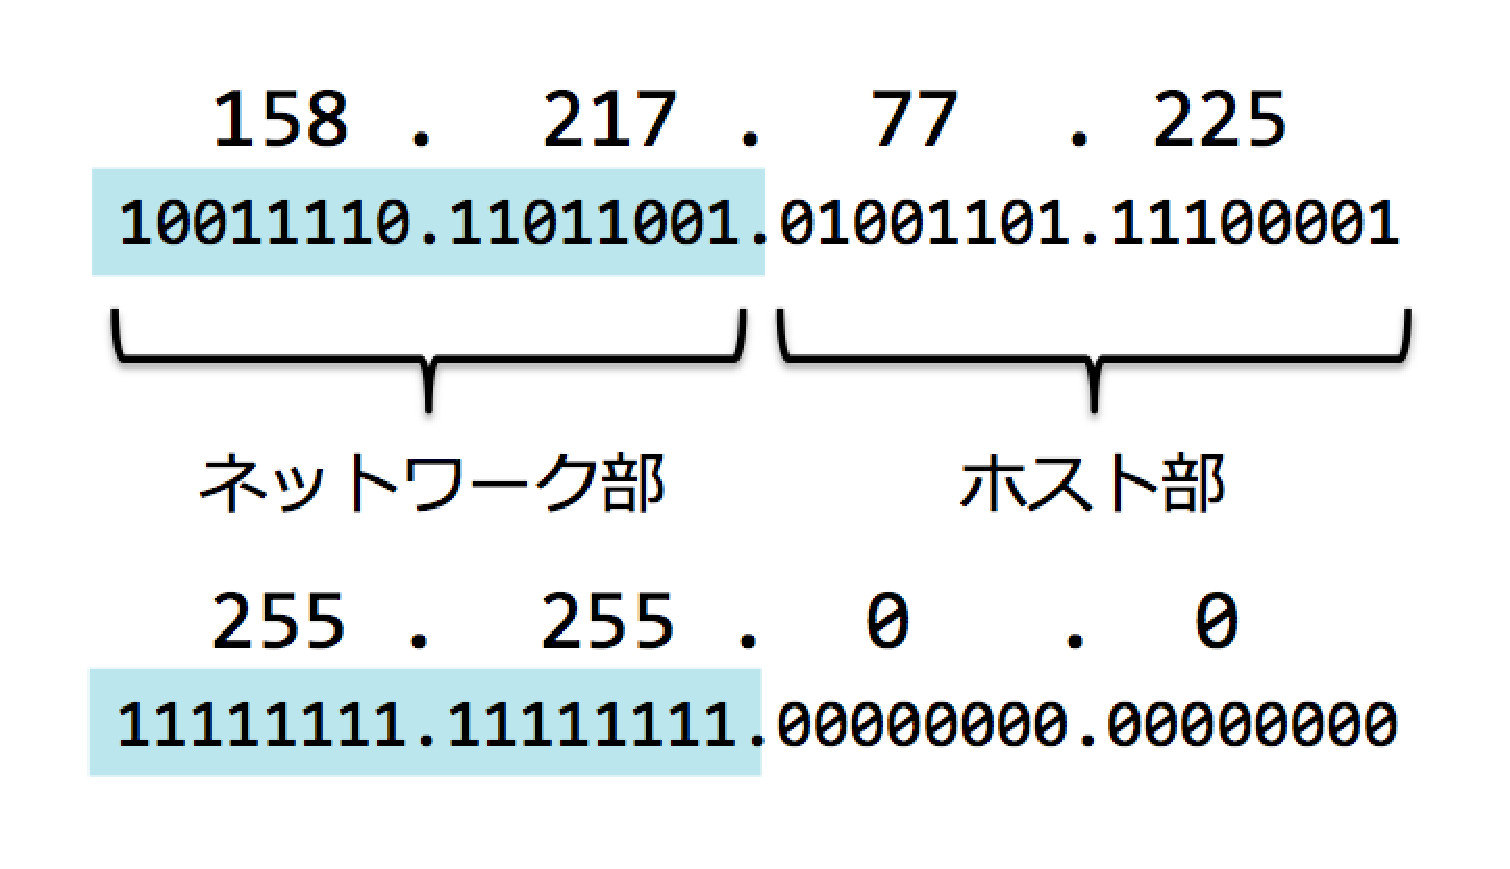
\includegraphics[width=82mm, bb=0 0 709 401]{netmask1.eps} 
  \end{center}
  \caption{ネットワーク部とホスト部}
  \label{fig:netmask1}
\end{figure}

IPアドレスはホストが属するネットワークを示す『ネットワークアドレス』と,機器を特定する『ホストアドレス』から構成される階層型アドレスである.図\ref{fig:netmask1}の例では,「158.217.77.225は,158.217.0.0ネットワークにある77.225番の機器である.」と解釈することができる.何処(158.217.0.0ネットワーク)の誰(77.225番)という情報があれば,相手が自分と同じネットワークにいるのか,あるいは遠く離れたネットワークに居るのか,などを見分けることができるため,通信経路の探索が容易になる.

ネットワークアドレスは全ネットワーク内でユニークなものである必要があり,インターネットの場合ではNIC(Network Information Center)等の組織が企業やプロバイダに対してネットワークアドレスを割り振っている.一方,ホストアドレスは各ネットワークの管理者が任意の機器に割り振ることができ,そのネットワーク内でユニークなものでさえあれば良い.

\subsection{クラスフルアドレッシング}

先程の例(158.217.77.225)では,IPアドレスの左から16ビットをネットワークアドレスを示す『ネットワーク部』,残りのビットをホストアドレスを示す『ホスト部』としていたが,この境目はIPアドレスが属するアドレスクラス(表\ref{tab:ip_class})によって決定される.

\begin{table}[htb]
  \begin{center}
    \caption{アドレスクラス}
    \begin{tabular}{|c|c|c|c|c|c|} \hline
      クラス & アドレス範囲 & ネットワーク部 & ホスト数  & 用途 \\ \hline \hline
      A & 0.0.0.0 〜 127.255.255.255 & 8ビット & 16,777,214 & 大規模ネットワーク用  \\ \hline 
      B & 128.0.0.0 〜 191.255.255.255 & 16ビット & 65,534 & 中規模ネットワーク用  \\ \hline 
      C & 192.0.0.0 〜 223.255.255.255 & 24ビット & 254 & 小規模ネットワーク用 \\ \hline 
      D & 224.0.0.0 〜 239.255.255.255 & - & - & マルチキャスト用 \\ \hline 
      E & 240.0.0.0 〜 255.255.255.255 & -  & - & 実験用 \\ \hline 
    \end{tabular}
    \label{tab:ip_class}
  \end{center}
\end{table}

ネットワーク部とホスト部の境目を示すビット列(例. 255.255.0.0)のことを『ネットマスク』と呼び,アドレスクラスを元にネットマスクを決定する方式を『クラスフルアドレッシング』と呼ぶ.

IPアドレスは32ビット固定であるため,ネットワーク部が大きくなればホスト部は小さくなり,そのネットワークに割り振れるホストの数は少なくなる.逆に,ネットワーク部が小さくなればホスト部は大きくなり,そのネットワークに割り振れるホストの数は多くなる.しかし,クラスAの場合では割り振れるホストの数が16,777,214台にもなり,一つのネットワークとして管理するにはあまりにも巨大になってしまうという問題がある.対応策として,次の項で説明する『サブネット』などの手法が用意されている.

\subsection{サブネット}
クラスフルアドレッシングのようなIPアドレスの分類はネットワークの規模に応じてIPアドレスを使い分けるために決められたものである.しかし,IPアドレスの値による固定的なネットマスクの分割ではあまり柔軟にネットワークを構築することはできず,クラスAやクラスBのネットワークの場合にはネットワークがあまりにも巨大になってしまう.

そこで,各ネットワークの管理者が自由にネットワークアドレスとホストアドレスを決定できるようにするために『サブネット分割』という手段が用いられる.既存のネットワークをさらに小さなネットワークに区切り,それを『サブネット』として扱うという手法である.いままではIPアドレスを『ネットワーク部』と『ホスト部』の2つに分けていたが,サブネットに区切った場合,IPアドレスは『ネットワーク部』,『サブネット部』,『ホスト部』の3つに分割されることになる(図\ref{fig:netmask2}).このとき,サブネット部の境目を示すビット列(例. 255.255.255.0)のことを『サブネットマスク』と呼ぶ.

\begin{figure}[htb]
  \begin{center}
    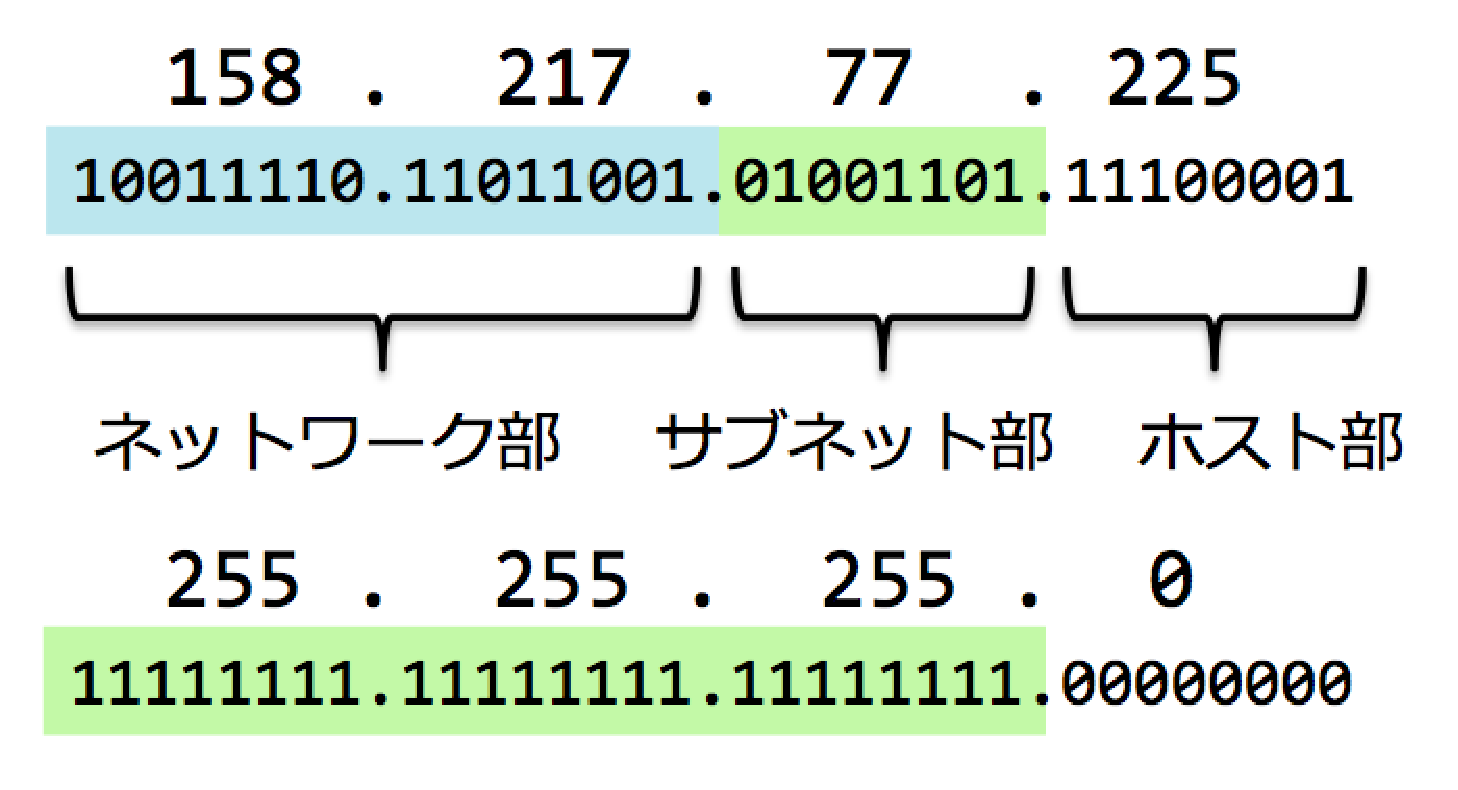
\includegraphics[width=82mm, bb=0 0 684 363]{netmask2.eps} 
  \end{center}
  \caption{サブネット分割}
  \label{fig:netmask2}
\end{figure}

アドレスクラスによって定められたネットマスクではなく,ネットワーク管理者が決めた自由なネットマスク(サブネットマスク)を使うことにより,ネットワークの規模などに応じて柔軟にネットワークを構築できるようになる.しかし,サブネットを使ったネットワークではネットマスクが環境ごとに異なるため,サブネットマスクをIPアドレスと同時に表記する必要がある.

\begin{itembox}[c]{サブネットマスクの表記法}
サブネットマスクの表記法にはいくつかの種類がある.
\begin{itemize}
    \item 192.168.1.52/11111111.11111111.11111111.00000000
    \item 192.168.1.52/255.255.255.0
    \item 192.168.1.52/0xffffff00
    \item 192.168.1.52/24
\end{itemize}
これら4種類の表記法はどれも同じサブネットマスクを表している.ソフトウェアによって様々な表記が使われるので,どれが出てきても意味が分かるようにしよう.
\end{itembox}

\subsection{予約済みアドレス}
IPアドレスの中にはどのホストにも割り振ることができない特別なアドレスが存在し,これらのアドレスのことを『予約済みアドレス』と呼ぶ.以下に各ネットワークごとに存在する2種類の予約済みアドレスについて説明する.

\begin{screen}
\begin{description}
 \item[ネットワークアドレス]\mbox{}\\ 
	    ホストアドレスのビットが全て0になるアドレス.これはネットワークそのものを表すアドレスであり,特定の機器ではなくネットワークそのものを指定したい場合に利用する.\\
 \fbox{例: 158.217.0.0(10011110.11011001.00000000.00000000)}
 \item[ブロードキャストアドレス]\mbox{}\\
	    ホストアドレスのビットが全て1になるアドレス.ネットワーク内の全てのホストを表すアドレスとなる. ネットワーク内の全ての機器に対してデータを送信したい場合に利用する.\\
\fbox{例: 158.217.255.255(10011110.11011001.11111111.11111111)}	    
\end{description}
\end{screen}

各ネットワークは必ずこれら2つの予約済みアドレスを持つため,ホスト部が\(n\)ビットだとするとホストに割り振れるアドレスは\(2^n-2\)個となる.予約済みアドレスはこれが全てではなく,他にもループバックアドレス(127.0.0.1)やプライベートアドレスといった特別なアドレスが予約されている.

\subsection{ifconfig/ipconfig}
ifconfig/ipconfigはIPネットワーク設定を確認したり,再設定したりするときに使うコマンドである.ネットワーク関係のコマンドとして最も頻繁に使われるものの一つで,ネットワーク管理には欠かせないコマンドである.情報の見方を是非頭に入れておこう.

Macではifconfigをターミナルから,Windowsではipconfigをコマンドプロンプトから実行する.

\begin{screen}
\begin{description}
 \item[Mac(ifconfig)]\mbox{}\\ 
  \begin{center}
    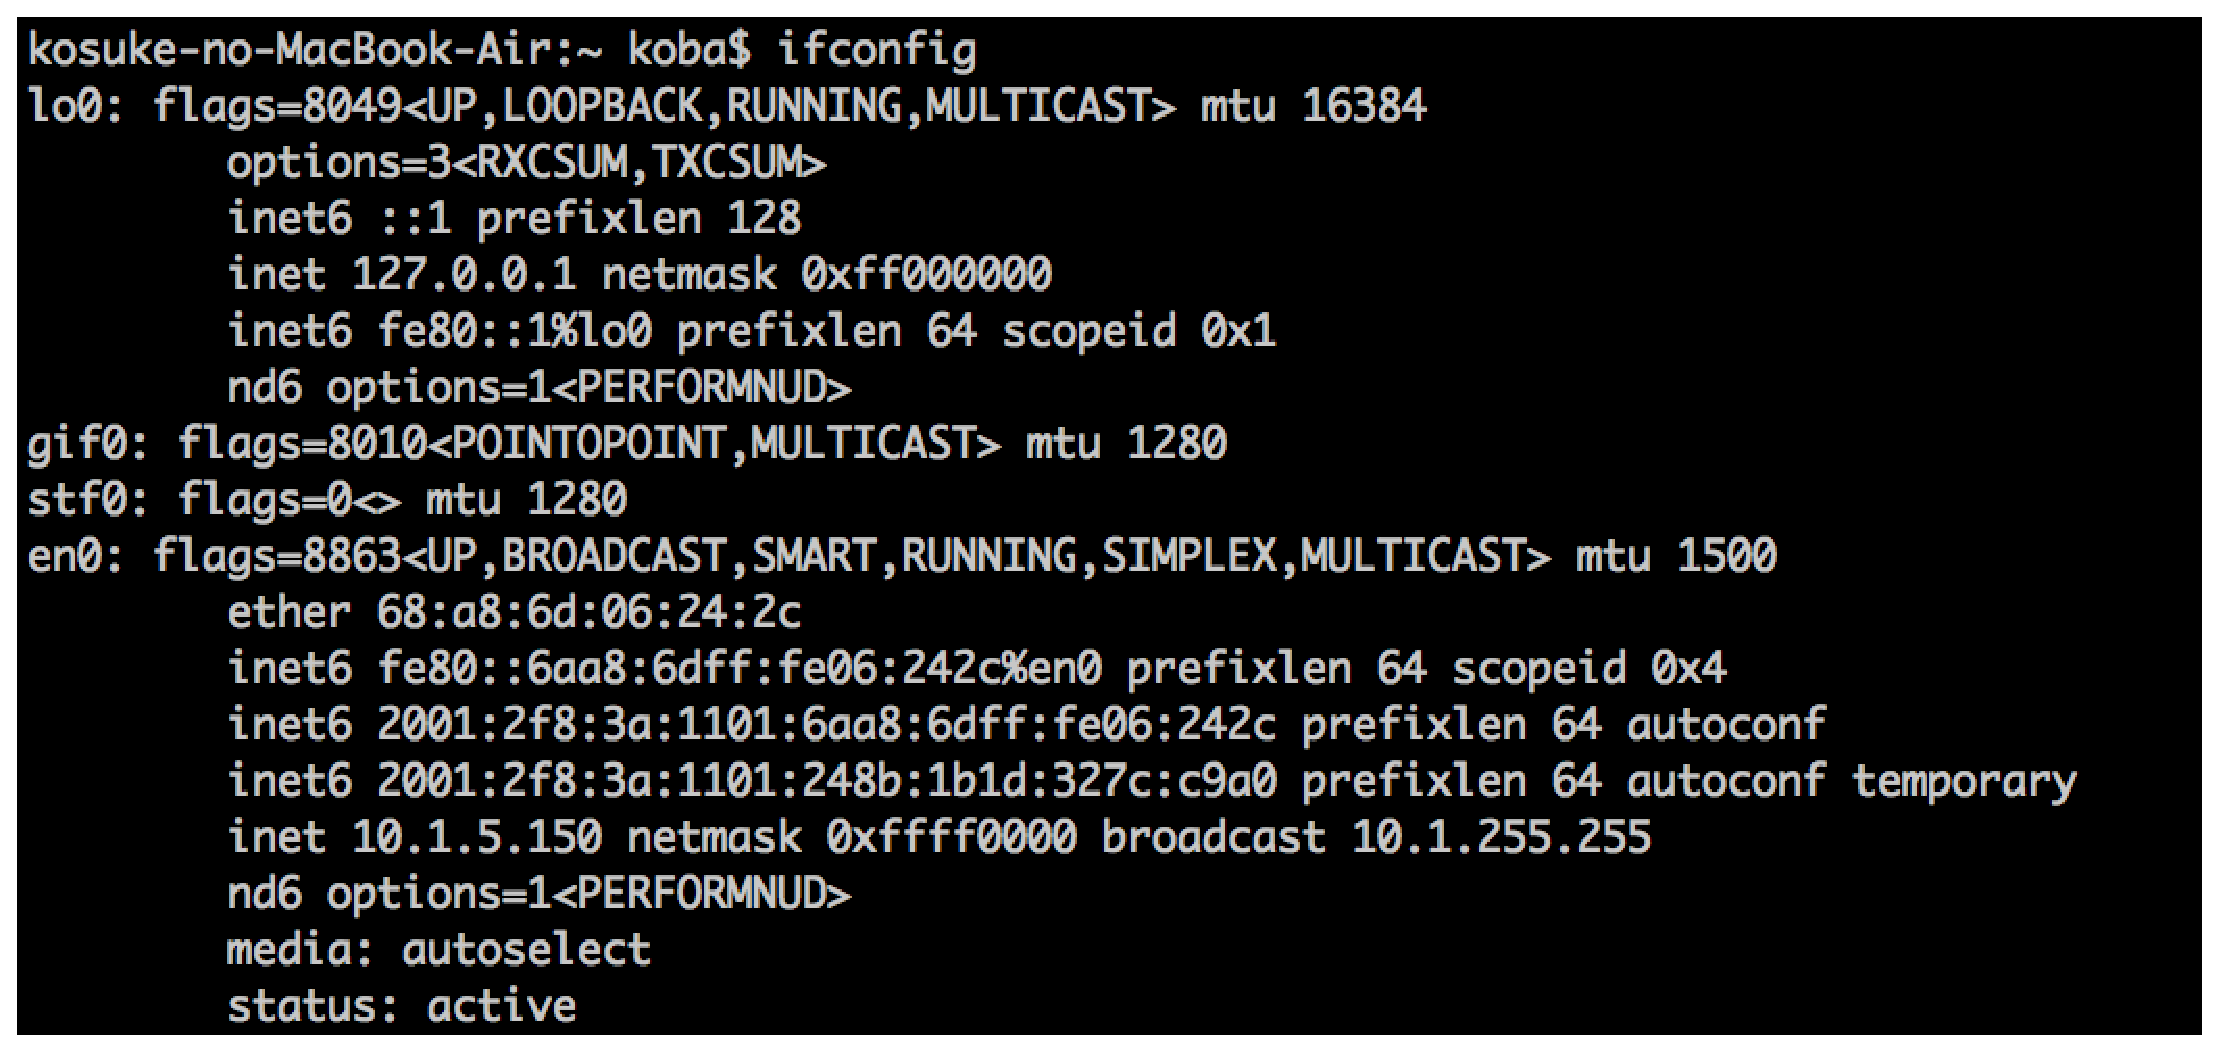
\includegraphics[width=140mm, bb=0 40 1049 469]{ifconfig.eps} 
  \end{center}
  上の実行例ではen0がネットワークに繋がる機器(NIC)となっている.etherの項にはMACアドレス,inet6の項にはIPv6についての情報が記載されている.\\
  IPアドレス(IPv4)についての情報はinetから始まる行に記載されている.\fbox{inet 10.1.5.150}は機器に割り振られたIPアドレスを表し,\fbox{netmask 0xffff0000}はサブネットマスクを表している.\\
 \item[Windows(ipconfig)]\mbox{}\\
     \begin{center}
    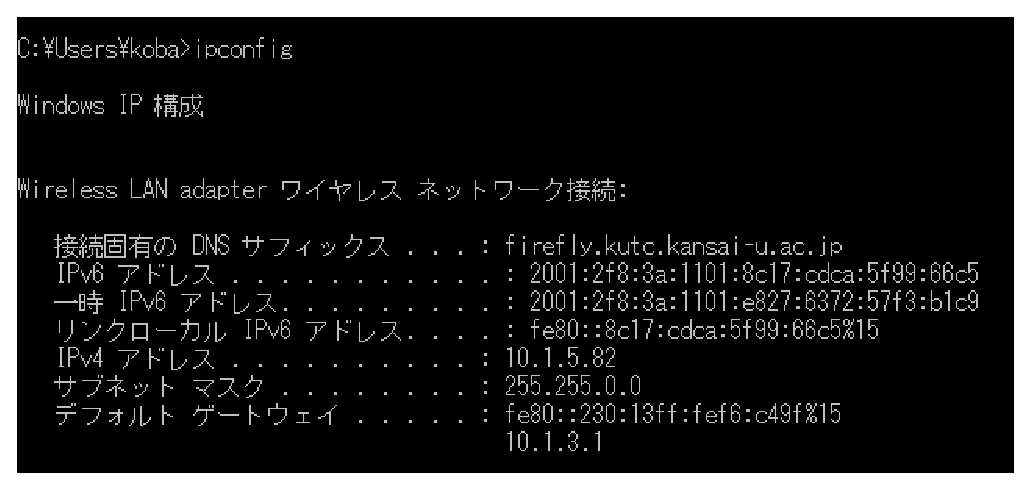
\includegraphics[width=138mm, bb=0 0 478 212]{ipconfig.eps} 
  \end{center}
  IPアドレス(IPv4)についての情報はIPv4アドレスから下の項に記載されている.\fbox{IPv4アドレス…: 10.1.5.82}は機器に割り振られたIPアドレスを表し,\fbox{サブネットマスク…: 255.255.0.0}は見ての通りサブネットマスクを表している.
\end{description}
\end{screen}

\subsection{DNS}
DNS(Domain Name Service)はIPアドレスとドメイン名の対応付けを行うサービスである.ドメイン名からIPアドレスを問い合わせること(正引き)と,IPアドレスからドメイン名を問い合わせること(逆引き)の両方を行うことができる.インターネットを利用する上でなくてはならない存在であり,現在のインターネットにとって必要不可欠なシステムの一つである.

ブラウザでWebページを閲覧するとき,ブラウザはIPアドレスを使ってWebサーバと情報のやり取りを行っている.しかし,ブラウザを利用しているユーザが直接IPアドレスを入力することは少ない.ユーザが入力するのは多くの場合,IPアドレスと比べて記憶し易いURI(例. https://www.firefly.kutc.kansai-u.ac.jp/xoops/)である.

URIからプロトコル名(https://)とディレクトリ名・ファイル名(/xoops/)を取り払ったものをドメイン名,厳密にはFQDN(完全修飾ドメイン名)と呼ぶ.ブラウザはこのドメイン名を使って目的のWebページのIPアドレスをDNSサーバに対して問い合わせ,IP通信を行っている.

ネットワークの設定の際にはDNSサーバ(及びセカンダリDNSサーバ)のIPアドレスが求められる.小林ゼミではDNSサーバ(10.1.3.21,10.1.3.80)を運用しており,ゼミ内ネットワークを使用する際にはこれらのDNSサーバのIPアドレスを設定する必要がある.

\subsection{FQDN}
FQDNとドメイン名は混同されがちであるが,厳密には異なるものである.ドメイン名はサーバが存在するネットワークを特定するための文字列であるが,FQDNはさらにホスト名をドメイン名に加えたものである.そのため,FQDNはホスト名とドメイン名に分割して考えることができる(図\ref{fig:URI_hostdomain}).

\begin{figure}[htb]
  \begin{center}
    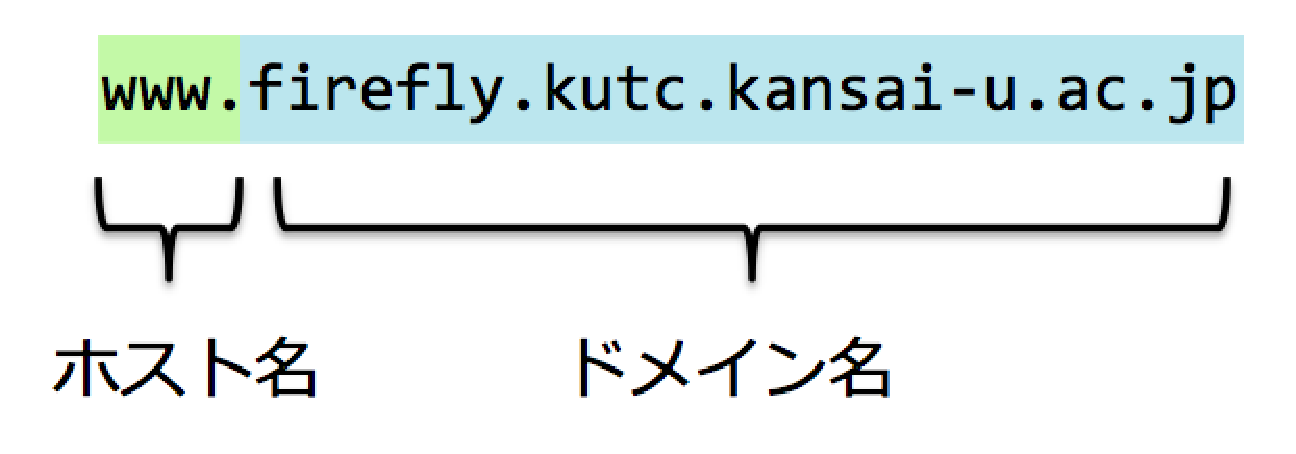
\includegraphics[width=100mm, bb=0 0 606 202]{hostdomain.eps} 
  \end{center}
  \caption{ドメイン名とホスト名}
  \label{fig:URI_hostdomain}
\end{figure}

FQDNは階層型の構造となっており,www.firefly.kutc.kansai-u.ac.jpは「日本(jp)の大学(ac)の関西大学(kansai-u)の高槻キャンパス(kutc)の小林ゼミ(firefly)のWebサーバ(www)」という意味である.

システムによっては末尾にドット(.)をつけることを表記のルールとしていることもあるので(例: www.firefly.kutc.kansai-u.ac.jp.)注意が必要である.

\subsection{nslookup}
nslookupはDNS問い合わせを手動で実施するためのコマンドである.任意のDNSサーバを指定して問い合わせを行うことも可能であり,DNSのトラブルシューティングでは非常に良く使用される.ネットワーク関連の基本的コマンドの一つである.\\

\fbox{nslookup [FQDNまたはIPアドレス] [任意のDNSサーバ名またはIPアドレス]}\\

一番基本的なnslookupの使い方は,引数にFQDNを指定してnslookupを起動することである.この使い方を『正引き』と呼び,FQDNに対応するIPアドレスがDNSサーバから取得される(図\ref{fig:nslookup1}).

\begin{figure}[htb]
  \begin{center}
    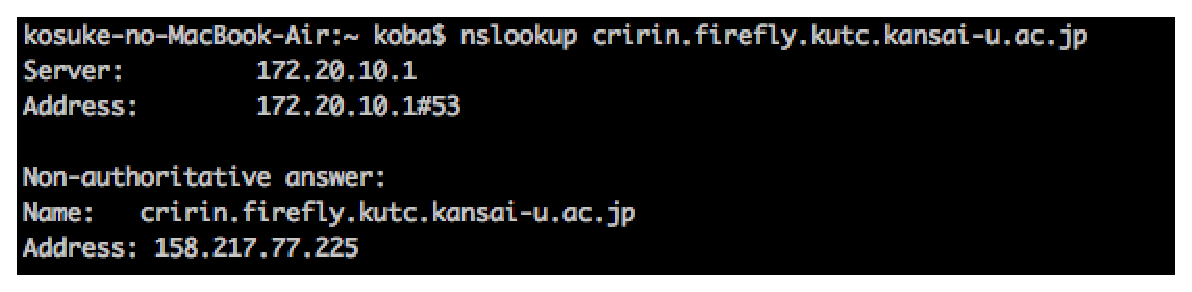
\includegraphics[width=150mm, bb=0 0 556 124]{nslookup1.eps} 
  \end{center}
  \caption{正引き}
  \label{fig:nslookup1}
\end{figure}

次によく使われるnslookupの使い方は,引数にIPアドレスを指定してnslookupを起動することである.この使い方を『逆引き』と呼び,IPアドレスに対応するFQDNがDNSサーバから取得される(図\ref{fig:nslookup2}).

\begin{figure}[htb]
  \begin{center}
    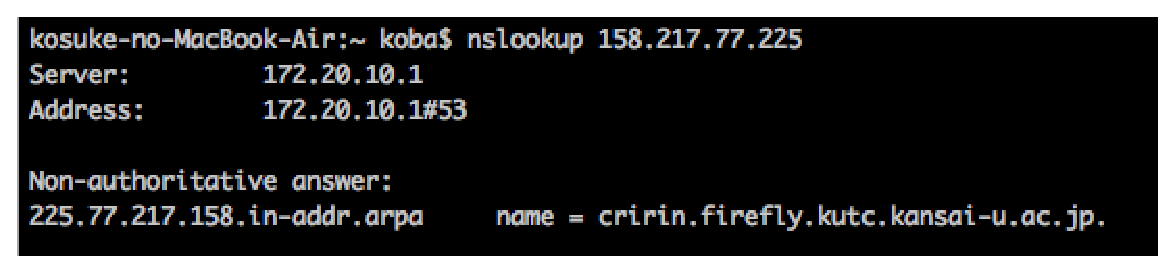
\includegraphics[width=150mm, bb=0 0 556 124]{nslookup2.eps} 
  \end{center}
  \caption{逆引き}
  \label{fig:nslookup2}
\end{figure}

